\documentclass[aspectratio=169, 12pt, a4paper, hyperref={pdfauthor={Alexandre MARIN}, pdfkeywords={IFPEN, Delaunay, Voronoi, mesh generation}, colorlinks=true, linkcolor=purple, urlcolor=blue, citecolor=magenta}]{beamer}
\usepackage[utf8]{inputenc}
\usepackage[french]{babel}
\usepackage[T1]{fontenc}
\usepackage{amsmath}
\usepackage{amsfonts}
\usepackage{amssymb}
\usepackage{graphicx}
\usepackage{xcolor}
\usepackage{tikz}

\usepackage[francais]{IFPENPresentation}
\usepackage{array}
\usepackage{multirow}
\usepackage{ctable}

\usepackage[defaultbib]{bibtopic}
%\renewcommand{\thesection}{\arabic{section}}

\graphicspath{{figures/}}


\begin{document}

\begin{frame}
\institute[]{
IFP \'Energies nouvelles\\ 
Direction Sciences et Technologies du Numérique -- Département Informatique Scientifique\\
1-4 avenue du Bois-Préau \textsc{RUEIL-MALMAISON}}
\date{2 novembre 2020}
\author{\small Alexandre \textsc{MARIN}\\ { Master Mathématiques et Applications Sorbonne Université\\ Parcours Ingénierie Mathématique\\ Majeure Ingénierie Mathématique Pour l'Entreprise}}
\title{Développement d’une bibliothèque de structures et algorithmes pour un mailleur polyédrique}
\subtitle{\small Soutenance de fin de stage\\ Encadrants :\\ Laurent \textsc{Astart}, Alexandra \textsc{Bac}}
\maketitle
\end{frame}

\begin{Energie}{Plan}
\tableofcontents
\end{Energie}

\section{Introduction}

\subsection{Présentation d'IFPEN}
\begin{Energie}{Brève présentation d'IFPEN}
\begin{itemize}
\item un EPIC
\item $\approx 50$\% de son budget issu de l'\'Etat
\item un groupe employant $1\ 600$ salariés
\item conçoit et développe des procédés, équipements et logiciels relatifs à quatre domaines :
\begin{itemize}
\item la mobilité durable
\item les énergies renouvelables
\item les hydrocarbures responsables
\item \textcolor{red}{le climat/environnement}
\end{itemize}
\end{itemize}
\end{Energie}

\subsection{Objectifs}
\begin{Energie}{Objectifs}

Premier objectif : faire un travail bibliographique et développer des structures de données et algorithmes pour un mailleur polyédrique 3D, censé être adapté à la simulation d'écoulements dans le sous-sol.
\\[1cm]
Objectif retenu : s'approprier des concepts sur la génération de maillages 2D et mettre en \oe{}uvre certains algorithmes en programmant une bibliothèque logicielle.
\end{Energie}

\subsection{Calendrier}
\begin{Energie}{Déroulement du stage}
{\renewcommand{\arraystretch}{1.5}
\renewcommand{\tabcolsep}{0.2cm}
\begin{tabular}{c|p{12cm}}
Juillet & Installation, programmation en C++ d'une structure en demi-arêtes et d'algorithmes de génération de maillages Delaunay\\
Août & Réorganisation du code, génération de maillages Delaunay contraints, tests\\
Septembre & Création de diagrammes de Voronoï, rédaction du rapport\\
Octobre & Seconde étude bibliographique\\
\end{tabular}}
\end{Energie}

\section{Mission du stage}

\subsection{Travail effectué}
\begin{Energie}{Première étude bibliographique}
\bibliographystyle{plain}
\begin{btSect}{../report/doc}
\btPrintNotCited
\end{btSect}
\label{biblio}
\end{Energie}

\begin{Energie}{Bibliothèque logicielle programmée (C++)}
\begin{center}
\usetikzlibrary {shapes.geometric}
\begin{tikzpicture}[fill=blue!20]
%\draw[help lines] (-1,-2) grid (6,3);
\path (0,0)
(10,0) node(c) [rectangle,draw,fill] {GeometricCore}
(5,0) node(d) [rectangle,draw,fill] {MeshCore}
(2,2) node(e) [rectangle,draw,fill] {MeshIO}
(2,0) node(f) [rectangle,draw,fill] {Delaunay}
(2,-2) node(g) [rectangle,draw,fill] {Voronoi}
(2,-4) node(h) [rectangle,draw,fill] {Test};
\draw[thick, ->] (d) |- (c);
\draw[thick,->] (h) -| +(-2,0) |- (f) ;
\draw[thick,->] (h) -| +(-2,0) |- (e) ;
\draw[thick,->] (h.north) -- (g) ;
\draw[thick,->] (h.east) -- (d) ;
\draw[thick,->] (h.east) -- (c) ;
\draw[thick,->] (e) -- (d) ;
\draw[thick,->] (f) -- (d) ;
\draw[thick,->] (g) -- (d) ;
\draw[thick,blue,->] (f) .. controls +(down:1.5cm) .. (c);
\draw[thick,blue,->] (g.east) .. controls +(right:1.5cm) .. (c);
\end{tikzpicture}
\label{archi}

Architecture du projet (sous QtCreator)
\end{center}
\end{Energie}

\begin{Energie}{Seconde étude bibliographique}

Elle concerne

\begin{itemize}
\item des structures de données représentant des maillages 3D polyédriques :
\begin{itemize}
\item demi-arêtes
\item cartes combinatoires
\item $\mathcal{G}$-cartes
\item $n$-cartes
\end{itemize}
\item des méthodes de génération de maillages polyédriques pour des simulations en géosciences :
\begin{itemize}
\item par résolution de problèmes d'optimisation
\item par des algorithmes de raffinement
\end{itemize}
\end{itemize}
\end{Energie}

\subsection{Résultats}
\begin{Energie}{Résultats}
\begin{itemize}
\item structure en demi-arêtes pour maillages bidimensionnels
\item maillages polygonaux exportés dans $3$ formats (Delaunay, Voronoï) de domaines convexes ou non
\item temps de calcul diminué grâce à la structure d'arbre quaternaire
\end{itemize}
\end{Energie}

\begin{Energie}{\normalsize Exemple de complexe linéaire par morceaux à mailler}
\begin{center}

\includegraphics[scale=0.25, viewport=620 250 1550 950, clip]{odd_plc.jpg}
\end{center}
\end{Energie}

\begin{Energie}{\normalsize Triangulation de Delaunay contrainte correspondante}
\begin{center}
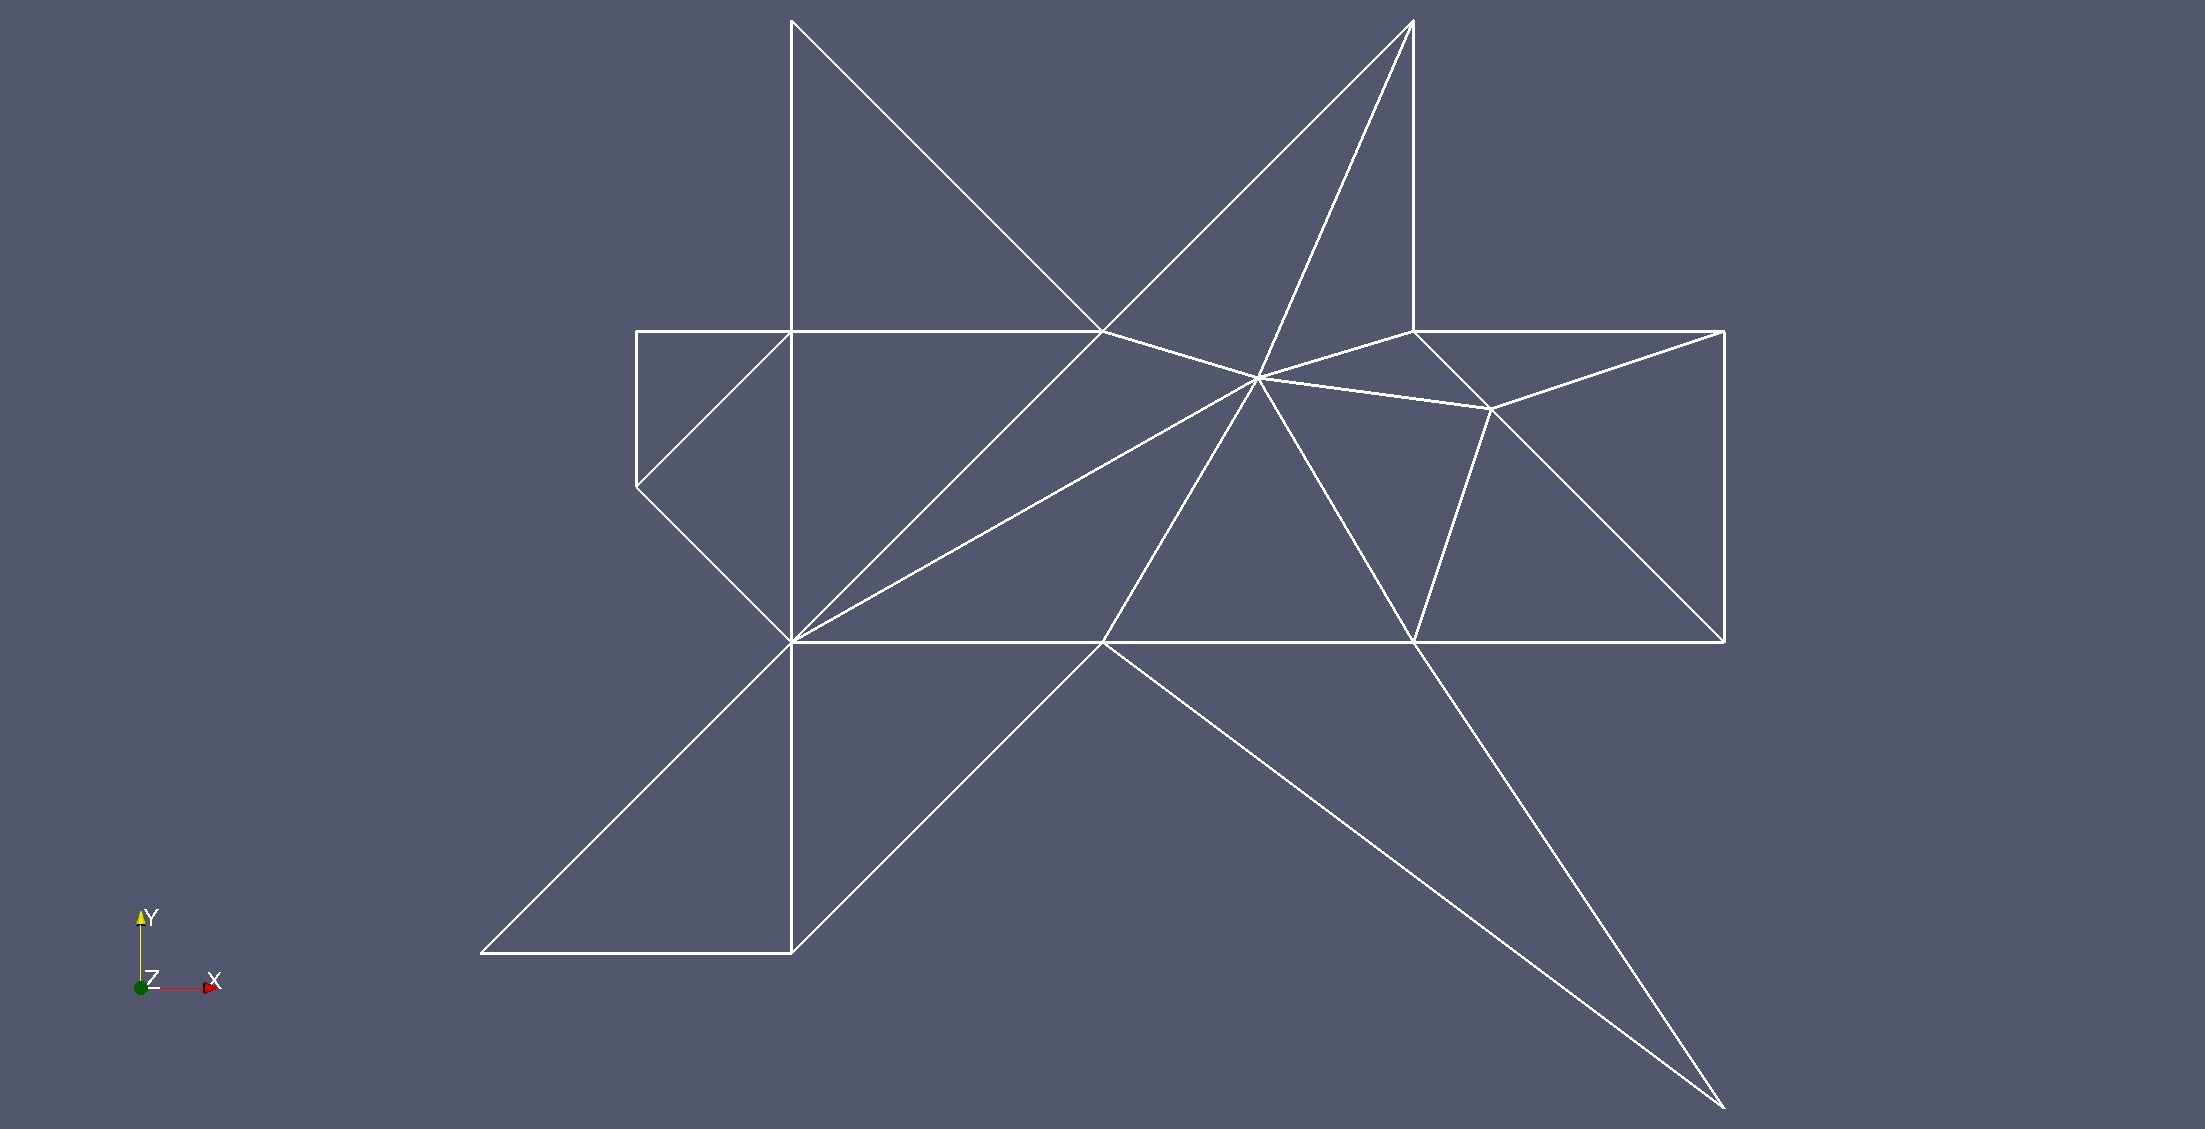
\includegraphics[scale=0.2, viewport=600 250 1750 1129, clip]{odd_cdt.jpg}
\end{center}
\end{Energie}

\begin{Energie}{\normalsize Un autre complexe linéaire par morceaux}
\begin{center}\vspace{-1cm}
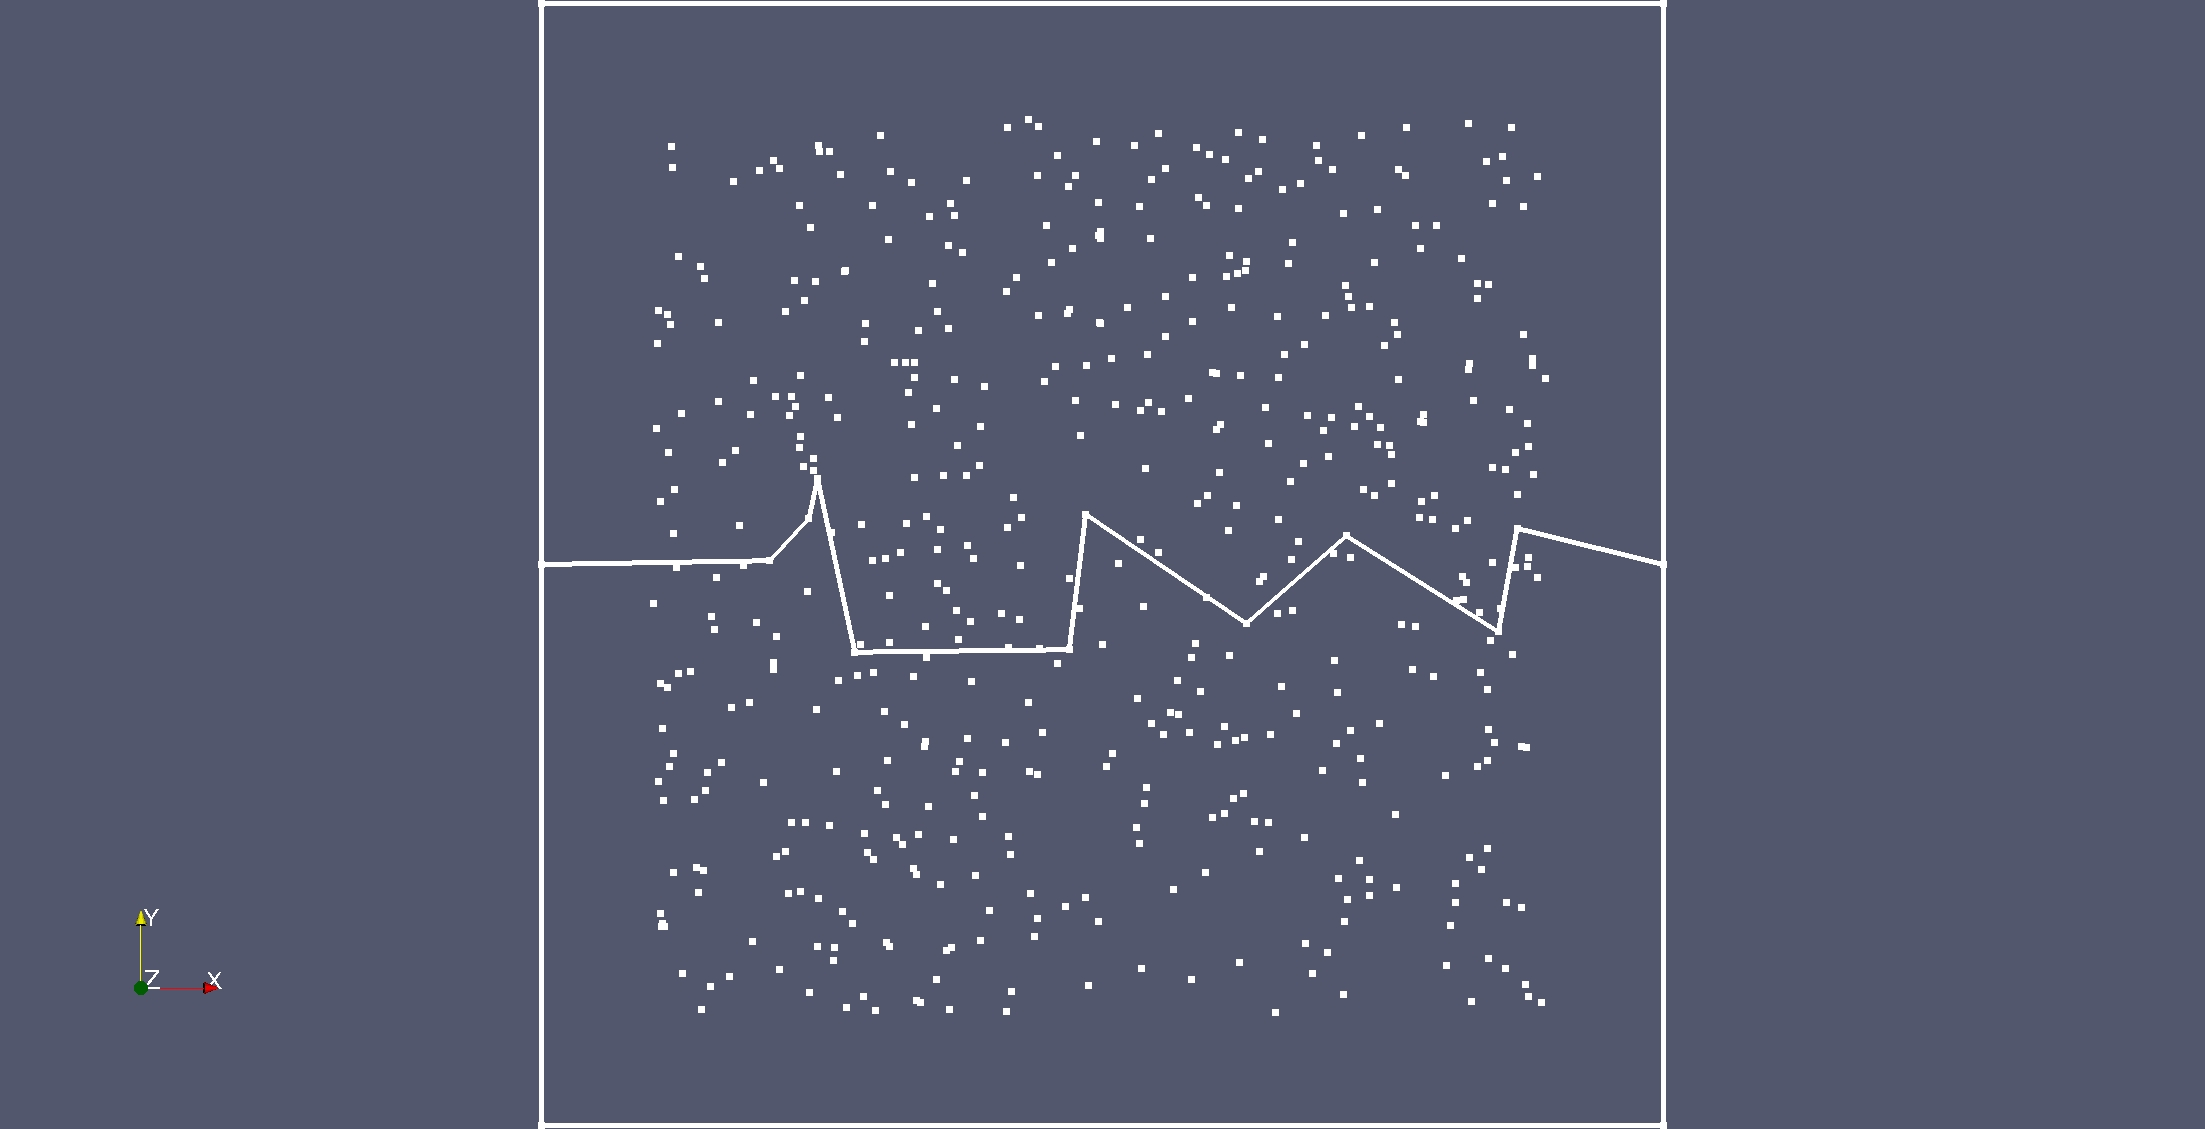
\includegraphics[scale=0.18, viewport=500 0 1700 1300, clip]{plc.jpg}
\end{center}
\end{Energie}

\begin{Energie}{\normalsize Diagramme de Voronoï correspondant}
\begin{center}\vspace{-1cm}
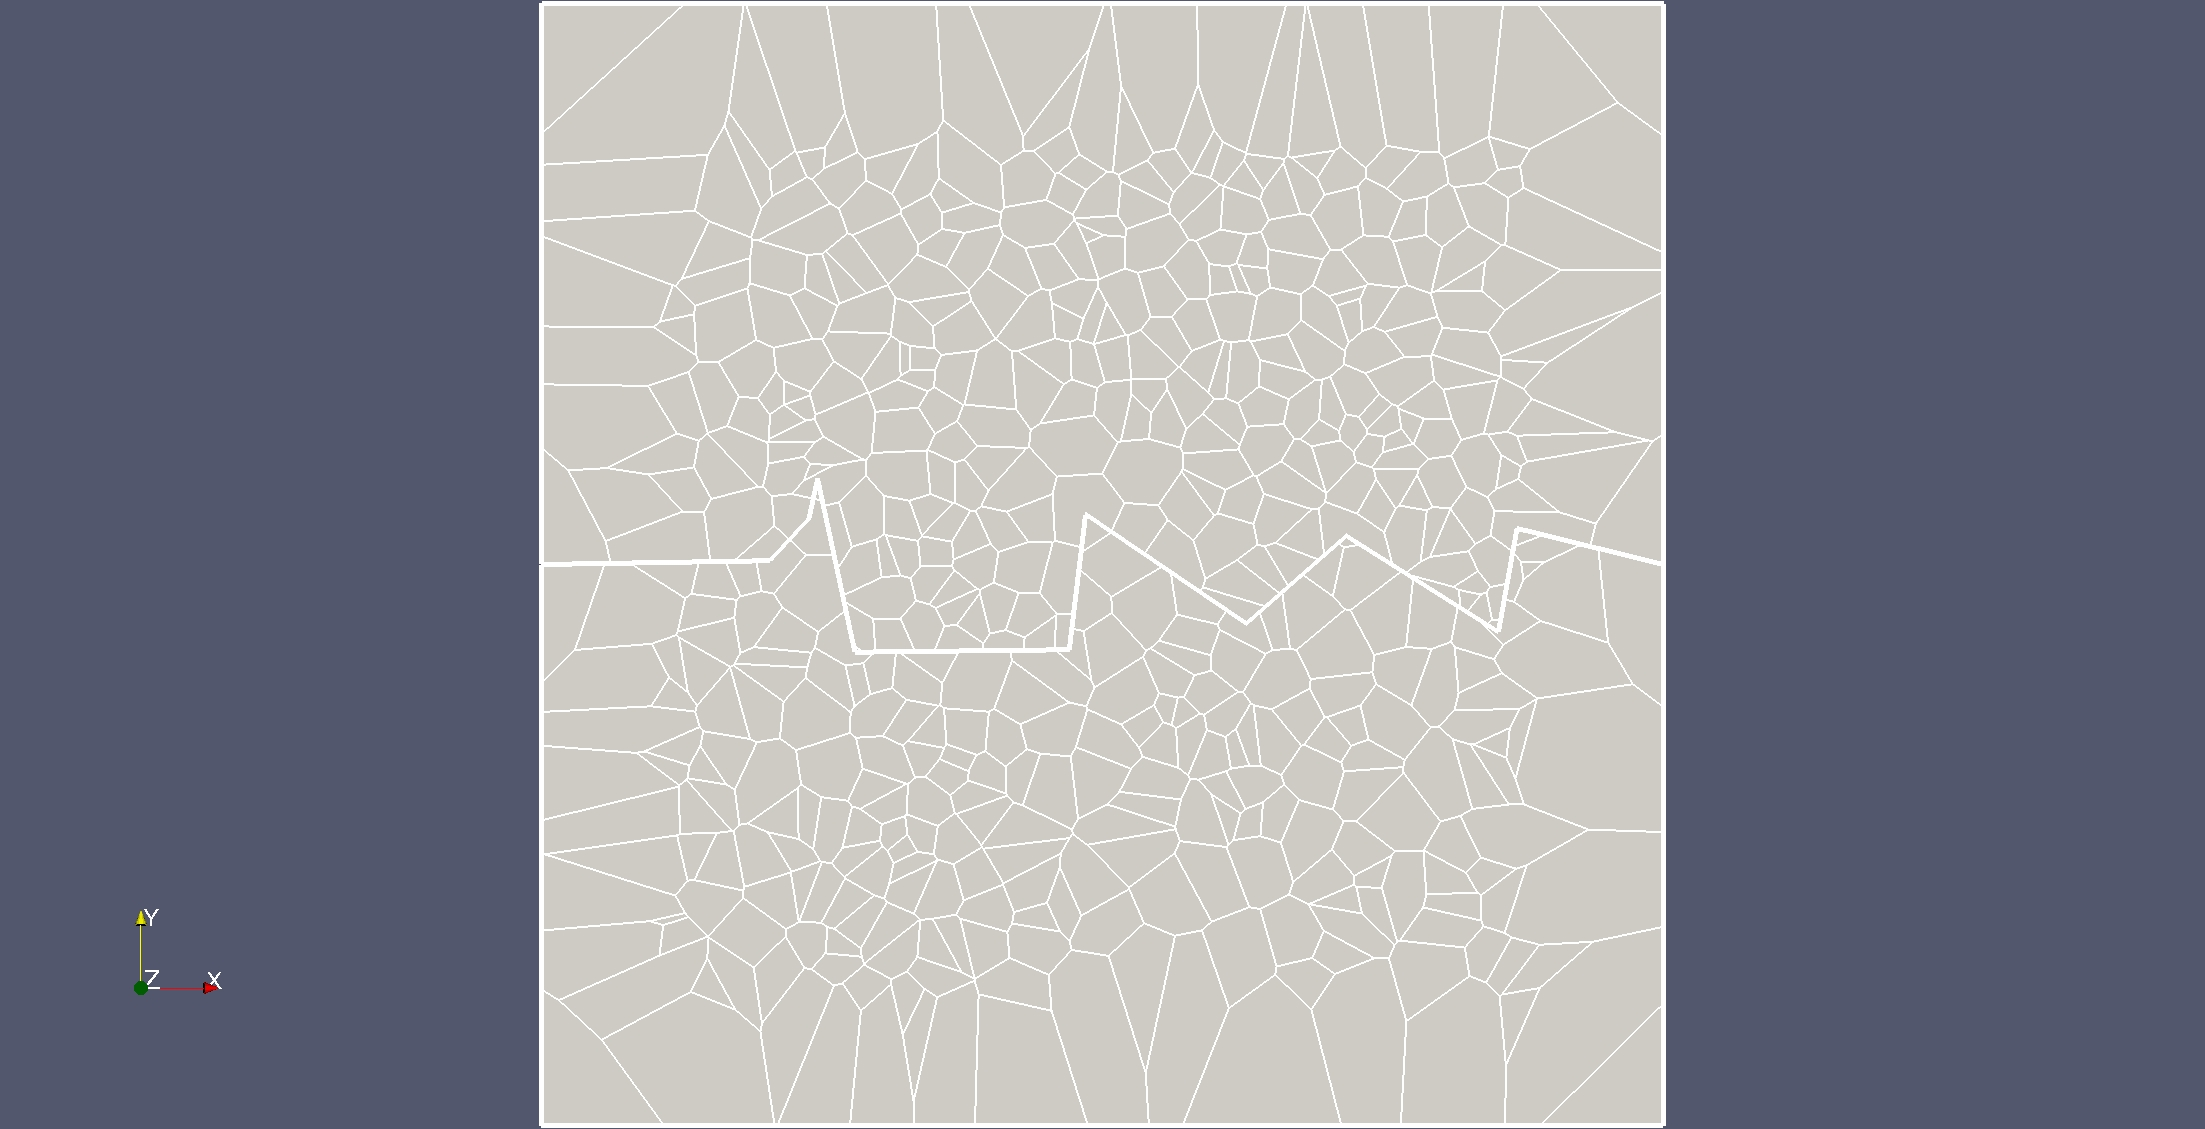
\includegraphics[scale=0.18, viewport=500 0 1700 1300, clip]{extended_vor.jpg}
\end{center}
\end{Energie}

\begin{Energie}{\normalsize Triangulation de Delaunay correspondante}
\begin{center}\vspace{-1cm}
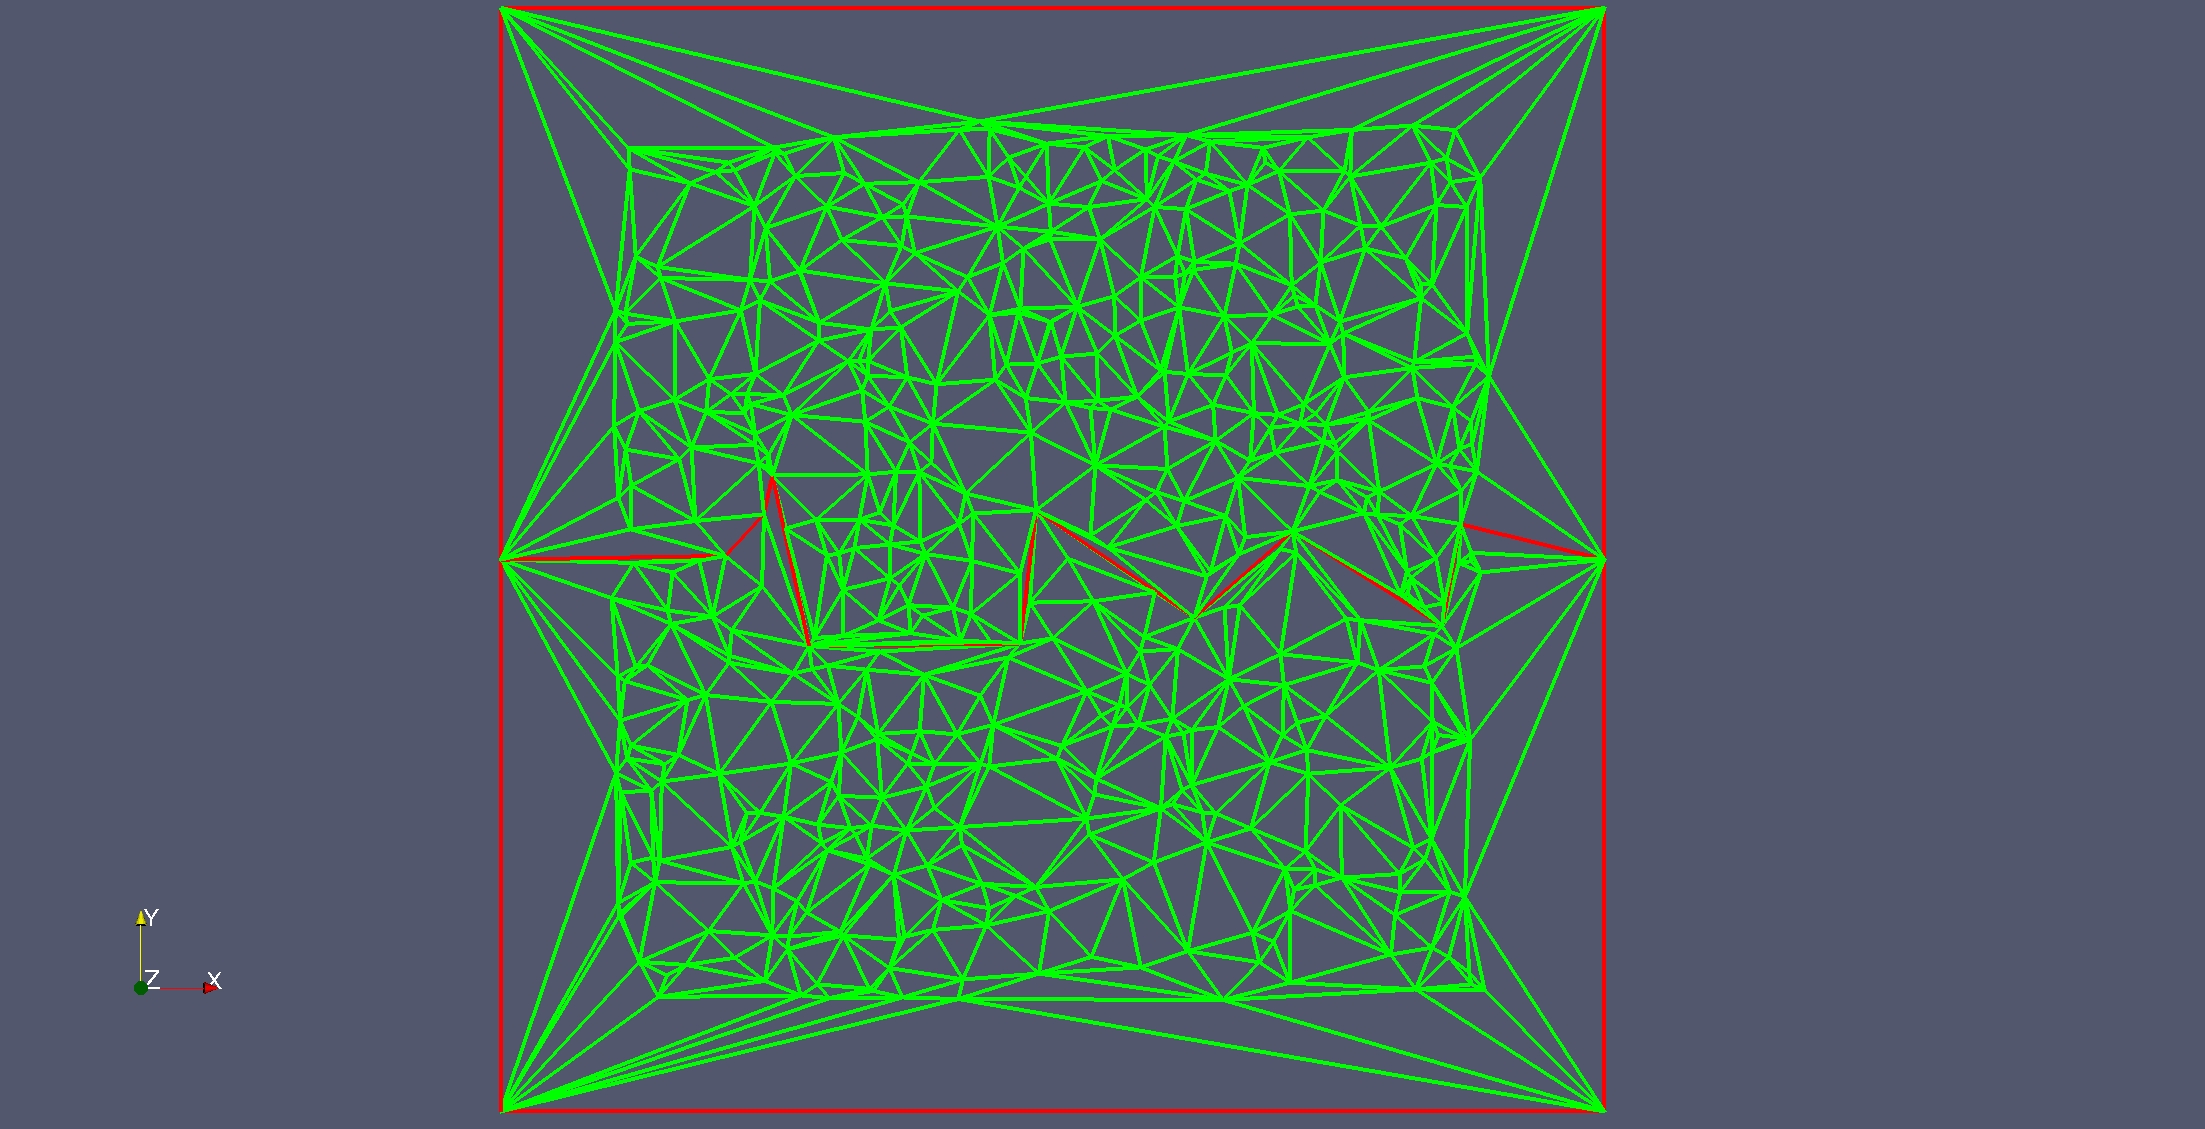
\includegraphics[scale=0.18, viewport=480 0 1630 1300, clip]{interfaceInSquare.jpg}
\end{center}
\end{Energie}

\subsection{Difficultés}

\begin{Energie}{Difficultés}
\begin{itemize}
\item différence entre théorie et pratique (arithmétique flottante)
\item conventions disparates des logiciels de visualisations (Paraview, CloudCompare, MeshLab)
\item existence de nombreux cas particuliers difficiles à couvrir avec des tests unitaires (intersections $\dots$)
\end{itemize}
\end{Energie}

\section{Conclusion}
\begin{Energie}{Conclusion}

Ce stage m'a permis de

\begin{itemize}
\item découvrir des concepts en génération de maillages, parfois pour les géosciences
\item de préparer la thèse qui suit : 
\begin{itemize}
\item difficultés
\item erreurs à ne pas reproduire
\item bibliographie
\end{itemize}
\end{itemize}
\end{Energie}

\makeByeSlide

\begin{Energie}{\small Bibliographie additionnelle}

{\tiny
\begin{btSect}{additional.bib}
\btPrintNotCited
\end{btSect}}
\end{Energie}

\end{document}